\section{Polynome}
\subsection{Definition}
Ein Polynom ist eine Funktion der Form:
\begin{align*}
    p(x) = a_n x^n + a_{n-1} x^{n-1} + \ldots + a_1 x + a_0
\end{align*}
\subsection{Nullstellen}
Im Polynom $f(x) = (x-1)(x+3)(x-8)^2(x-6)^3$ ist 8 eine Doppelnullstelle und 6 eine Dreifachnullstelle.\\
\subsubsection{Nullstellen Raten}
In Analyis 1 der ZHAW dürfen zudem Nullstellen geraten werden. Diese sind immer im folgenden Bereich: $\{-3,-2,-1,0,1,2,3\}$
\subsection{Horner-Schema}
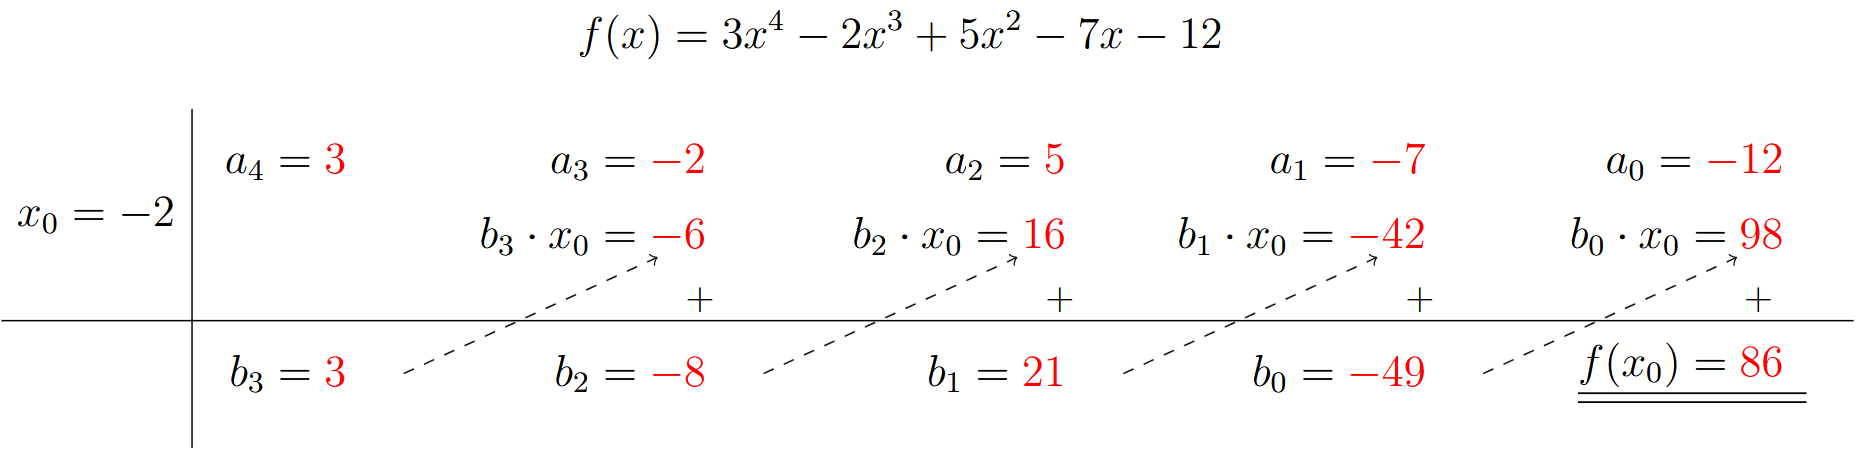
\includegraphics[scale=0.2]{horner}
\subsection{Polynomdivision}
\begin{center}
    \textbf{GOOD LUCK HOMIE}
\end{center}